\chapter{Introduction}\label{introduction}
In the last few decades, there has been a significant technological development in various fields.
Computing technology has advanced rapidly, with the introduction of faster and more powerful processors, and the widespread adoption of cloud computing.\newline
The Internet has also become an integral part of modern life, connecting people and devices across the globe; in addition, the development of faster and more reliable connectivity networks has made it possible to transfer and share data at an even faster rate.\newline
Mobile technology has grown exponentially, thanks to the adoption of smartphones and other mobile devices.\newline
One of the fields that has seen a substantial growth, due to the increasing availability and affordability of devices, sensors and other components, is the Internet of Things (IoT). The term IoT refers to the growing network of physical devices, vehicles, buildings and other items that are embedded with sensors, software and connectivity, which enables these \textit{Things} to collect and share data. These capabilities have the potential to bring significant benefits to society and economy, such as improving public services, increasing efficiency and productivity, and reducing costs.

This technological development is closely connected with the growth of distributed systems. As a consequence of the increase in computing power and the availability of fast and reliable networks, it has become possible to allow devices and systems to work together and share data, even when they are physically separated.

The general growth just discussed brought new challenges, such as the need of engineering complex software which has to take full advantage of the computational infrastructure available, taking in consideration the unpredictability of changes and the heterogeneity of communication required.

In order to face the new complexities it is necessary to rethink and renovate the process of software development.

\textit{Aggregate Programming} is a paradigm which aims to address these requirements. It allows for the easy manipulation of data across devices, making it possible to perform operation on the data of distributed systems, in a simple and efficient manner.\newline
This paradigm has been implemented in different programming languages and platforms: two of them are Protelis and Scafi. 
Both Protelis and Scafi presents strengths, but also weaknesses: in order to address those, a new framework can be a solution.

The work described in this thesis consists in the development of a new aggregate programming framework in Kotlin, which strengths are transparency, minimality and portability. 

\section{Context}
In this section it is going to be discussed in details the paradigm of Aggregate Programming, in order to provide the context of its development and an overview about how the paradigm works.

\subsection{Aggregate Programming}
Since the last few decades have witnessed technological advances, the traditional way of engineering software is, in some cases, suboptimal.
The systems developed are becoming more and more complex, with requirements that are difficult to achieve. 

These challenges are enhanced when coming to terms with distributed systems, because there is the need to handle the always increasing number of connected devices, that share and compute data.\newline
Some relevant complexities are the following \cite{distributed_systems_challenges}:
\begin{itemize}
    \item Scalability: as the number of devices in a distributed system grows, the coordination becomes increasingly complex. This requires the development of scalable algorithms and protocols that can handle large numbers of devices;
    \item Heterogeneity and interoperability: in a distributed system, devices may be made by different manufacturers and use different protocols, which can make it difficult for them to communicate with each other. The interoperability between heterogeneous devices and systems is a major challenge;
    \item Synchronization: devices are usually not connected to a common clock, which can make it difficult to synchronize their activities. This can lead to inconsistencies and errors within the system;
    \item Latency: the distance between devices in a distributed system can lead to high latency, which can affect the performance of the system. Managing and reducing latency is a challenge while coordinating numerous devices;
    \item Consistency: devices may have different views of the system state, which can lead to inconsistencies. Guarantee consistency across devices can be challenging and requires the development of distributed algorithms and protocols;
    \item Fault tolerance (or error control): devices may fail or become disconnected, which can disrupt the system. Ensuring fault tolerance and the ability to detect and recover from failures is essential in this kind of systems;
    \item Security and privacy: coordinating devices in a distributed system requires the sharing of sensitive information, which can create security risks.
\end{itemize}

Traditionally, the development in this kind of architectures is focused on the single device, instead of the system as a whole. This approach is not feasible when dealing with large-scale, decentralized and adaptive infrastructures, such as the one represented in Figure \ref{fig:iot_connected_things}.

\begin{figure}[!ht]
    \centering
    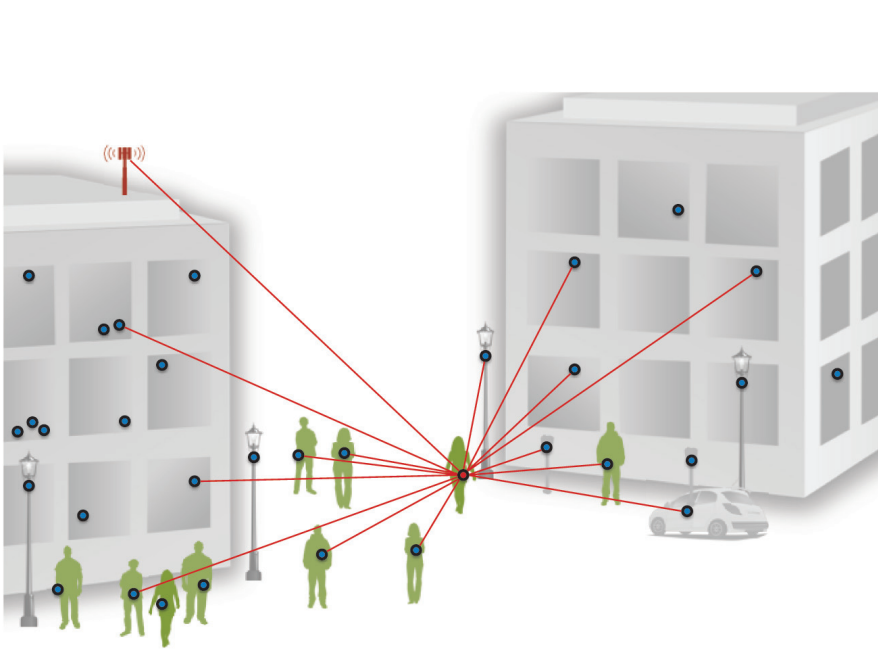
\includegraphics[scale=0.8]{document/chapters/1-introduction/images/iot_connected_things.png}
    \caption{Example of a real life environment, where heterogeneous devices have the possibility to communicate with each other wirelessly creating complex distributed systems. \cite{aggregate_programmig_iot}}
    \label{fig:iot_connected_things}
\end{figure}

Aggregate programming is a paradigm that focuses on the manipulation of complex data structures as a whole, rather than their individual components. The focus is on what a system is required to do, rather than on how is going to achieve it.\newline
This paradigm is closely related to the \textit{field calculus}, a mathematical framework for modeling and reasoning about distributed systems.\newline
Aggregate programming in combination with field calculus, provides a powerful tool for modeling, reasoning, and programming distributed systems. It allows for the efficient manipulation of large and complex data in distributed systems, and facilitates the representation of relationships and interactions between devices. It is a useful approach to adopt for IoT and other distributed systems where scalability, coordination, and security are critical concerns.

The basic concept used in aggregate programming is the \textbf{computational field}, which is a mathematical function that assigns a value to each point in a space, and it is used to represent and manipulate the state of a distributed system.

In order to explain better what a computational field is and how it is used, it is necessary to discuss the assumed computational model \cite{computational_fields_theory}.
Supposed a program P, it is executed by a network of devices, which is defined by a dynamic neighboring relationship. The computation of P can be analyzed by a local and a global point of view.
Considering the local perspective, P is computing on a round-based scheme in single devices. A round is executed in the following steps:
\begin{itemize}
    \item the device sleeps for a delta of time and at some point it wakes up;
    \item it retrieves information received from neighbors while it was sleeping. The messages sent by the neighbors are in fields, and they map the neighbor device identifier with the values computed;
    \item it gathers information about its context;
    \item it retrieves the information stored locally in the previous round about the context;
    \item it executes P, which might manipulate the data of the current context, the data retrieved in the previous round and the neighbors values;
    \item at the end of the execution of P, the device stores the current context's value in the local memory and sent the message to all the neighbors about the current computation;
    \item at the end of the round, the device returns to sleep, until another round begins.
\end{itemize}

On the other hand, the global point of view is the key that makes aggregate computing a powerful tool. In this case, the computation considers the entire network of interconnected devices as a single, unified entity.
The data is represented as a distributed space-time field evolution, which maps the computation events to values computed by devices.\newline
A computational field is a snapshot of the state of the distributed system's network at a certain moment in time, which maps device identifiers to their values.

The main constructs provided by the field calculus are the following:
\begin{itemize}
    \item \textbf{Rep-expression} $rep(e_0)\{(x)-> e\}$ \newline
    This is the repeat construct, and it represents the time evolution. This allows the field to change dynamically: if in the previous round the rep expression has not been evaluated, the initialization value is $e_0$, otherwise it is the value obtained in the last computation of rep;
    \item \textbf{Nbr-expression} $nbr\{e\}$\newline
    The neighboring is used to model the device-to-neighbor interaction. In order to do this, it is necessary to construct neighboring fields: in this data structure each event is associated to a value, that is mapped to a neighbor identifier and its last value computed. Using this construct it is possible for a device to understand its surrounding by manipulating the neighboring field obtained;
    \item \textbf{Branching} $if(e_0)\{e_1\} else \{e_2\}$\newline
    Branching causes a domain restriction, which means that devices compute $e_1$ only in the restricted domain where $e_0$ is true, otherwise they compute $e_2$. This behavior and its consequences will be discussed in details in Section \ref{section:alignment};
    \item \textbf{Function calls} $e(e_1, ..., e_n)$ \newline
    This construct model a function call where $e$ evaluates to a field of function values. 
\end{itemize}

As previously said, the data structures manipulated are distributed over space, and they evolve over time. These two aspects are handled, in the case of field calculus, by two separate constructs: the evolution in time is manipulated by \textit{rep-expression}, the space management, which provide neighbors interactions, is provided by the \textit{nbr-expression}.\newline
The use of time evolution and neighbor interaction operators in the traditional way leads to a slowdown in the efficient spread of information. This is due to the separation of state sharing (nbr) and state updates (rep), which requires information received through nbr to be stored through rep in the local memory of the device before it can be passed on during the next execution of nbr \cite{share_operator}. 

This limitation can be overcome by extending the field calculus with a new construct, which has been called \textbf{share} \cite{share_operator}. The share operator allows to observe the neighbors' field, updated the local values and sharing immediately the updated state in a single computation. It is possible to observe the differences between the behavior of the share operator and the combination of rep and nbr in Figure \ref{fig:share_operator_introduction}.

\begin{figure}[!ht]
    \centering
    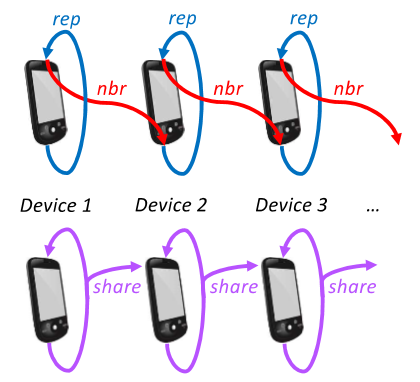
\includegraphics[scale=0.8]{document/chapters/1-introduction/images/share_operator_introduction.png}
    \caption{Comparison between the combination of rep-expression and nbr-expression, and the share construct \cite{share_operator}}
    \label{fig:share_operator_introduction}
\end{figure}

\subsubsection{Domain restriction: alignment}\label{section:alignment}
The expected consequence of a branch construct is to determine the portion of code that is going to be computed. In the field calculus, the branch construct has also an unusual behavior, which is called domain restriction.

Taking in consideration this portion of pseudocode
\begin{lstlisting}
    if (e0) {e1} else {e2}
\end{lstlisting}
it is possible to identify two different restricted subdomains: the first one it where e0 is true, which is going to be called $D_{true}$, the second one is defined by e0 equals to false, which is $D_{false}$.
For example, if a device is in the domain $D_{true}$, the following are the implications \cite{computational_fields_theory}:
\begin{itemize}
    \item it does not compute e2, which is the typical branch behavior;
    \item if e2 involves a nbr-expression, this is not going to be evaluated by the considered device. This means that the neighboring devices in $D_{true}$ can not obtain the value of this device for the nbr-expression in e2, because it has not been computed. Similarly, the nbr-expression in e1 evaluated by this device, is not going to be shared from $D_{false}$ to $D_{true}$;
    \item if the device evaluated e2 instead of e1 in its previous round, then all the rep-expressions in e2 are going to be computed using the initialization value.
\end{itemize}

Given this behavior, the result is that devices that operate in different subdomains are computing in isolation. This means that they can not communicate with each other, unless they are in the same domain. For this reason, this characteristic is called \textit{clustering}, which is an important feature: it allows restricting computations in subdomains in an easy and efficient way, which is extremely useful in many use-cases.

The domain restriction is a crucial trait of aggregate programming, and it introduces to a problem that has to be taken in consideration. Different devices that operate in a highly distributed system do not have a shared memory that can be used to keep track of the computation of each device. On the other hand, the domain restriction characteristic requires that each device has to communicate only with devices in the same subdomain, which means that they are computing the same operation.\newline
This is defined as the \textbf{alignment problem}, and it is necessary to explore all the information of the system in order to find a solution. First, it is important to keep in mind that each device has its own identifier, which can be used to define the author of a message. Second, when dealing with a computational field, such as when retrieving neighboring values using a nbr-expression, the device is currently computing the operation that it is actually looking for in the field.\newline
In order to explain this concept better, here is a snippet of pseudocode:
\begin{lstlisting}
    if (e0) {nbr(e1)} else {nbr(e2)}
\end{lstlisting}
When a device $\delta_1$ is in the domain $D_{true}$, it computes $nbr(e1)$: this means that it is retrieving from the neighbors that computed $e1$, while being evaluating $e1$ itself.\newline
Consequently, $\delta_1$ and the other devices have to be aligned in order to exchange information: they all are in the same subdomain, in which $e0$ is evaluated as true, and they are computing $nbr(e1)$.\newline
Given these concepts, it is possible to understand how to deal with the alignment problem: thanks to the current computational location of a device, it is possible to understand which values it is currently trying to retrieve, and, since each device has an identifier, the values can be mapped to those identifiers. Then, combining all the information together, a computational field is obtained.

\section{State of the art}
\subsection{Protelis}
\subsection{Scafi}
\subsection{FCPP}

\section{Motivation and goal}